\section{Objetivos}

\section{Fundamentação Teórica}

\section{Procedimentos}
\subsection{Exercício 1}
Considere um sistema em malha fechada com PID T(z) sendo:

\begin{figure}[!ht]
	\centering
	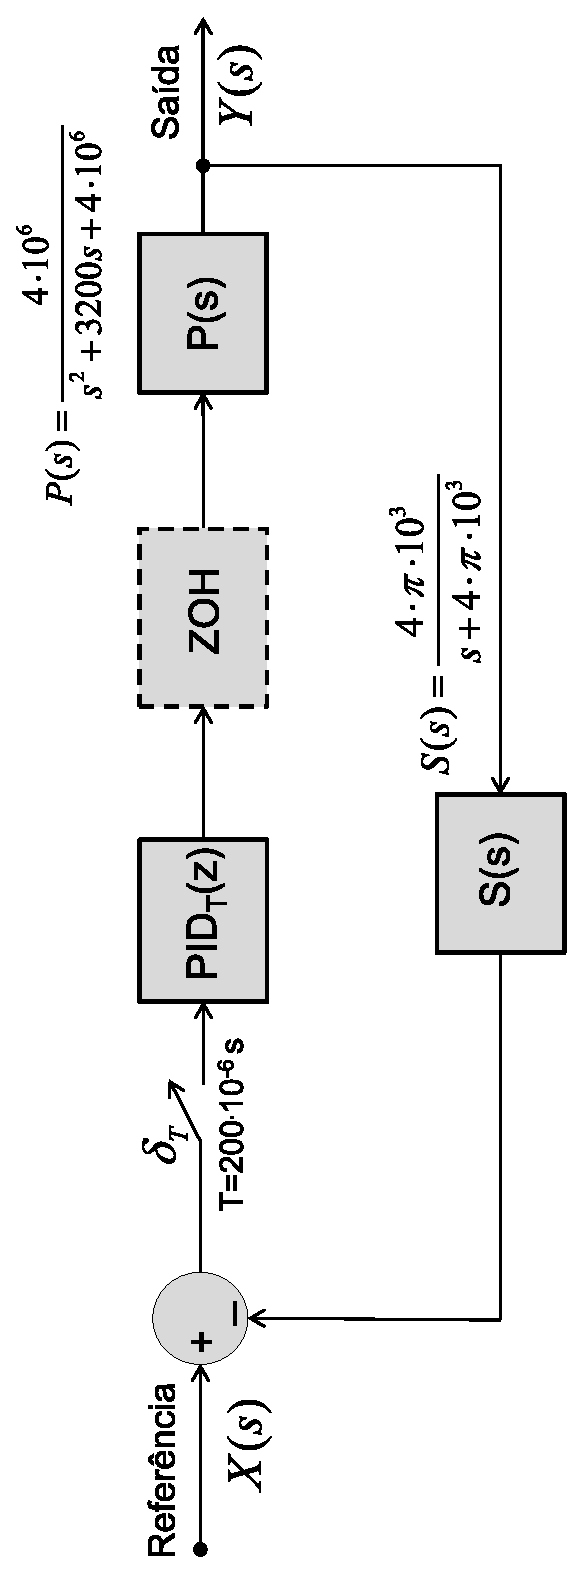
\includegraphics[scale = .5, angle =-90, frame]{Imagens/PID.eps}
	\caption{}
	\label{}
\end{figure}

Utilize simulações computacionais (Simulink\textregistered) para projetar ganhos para o controlador PID considerando a entrada um degrau unitário.

\subsection{Exercício 2}

Obtenha a função de transferência do PID de tempo discreto utilizando o método de discretização Forward para a parcela integral e considere Kp, Ki, e Kd como ganhos paralelos do controlador PID.

\subsubsection{Repita o Exercício 1 para esta função de transferência comparando os resultados de simulação de ambos os casos para os mesmos ganhos.}

\subsubsection{Inclua saturação na ação de controle em 150\% da referência e analise o comportamento do sistema de controle}

\subsection{Exercício 3}
Considerando o sistema descrito no exercício 2, desenvolva um script em Matlab para implementar o PID com os seguintes parâmetros.

\begin{itemize}
	\item Sinal de referência:
		Onda quadrada
		Amplitude $40~V_{pp}$
		Offset $0~V$
		Período $10ms$
	\item Controlador:
		PID ‘Digital’ (equação de diferenças)
		Saturação do PID (Sat = $0.98~V_{cc}$)
	\item Atuador: sinal PWM
		Resolução 8 bits (2n divisões)
		$V_{cc}=40~V$
	\item Ruído:
		Randômico
		Amplitude 2\% da saída
	\item Conversor A/D:
		Resolução 10 bits (2n níveis)
		Vin=0-5V
		T=200.10-6 s
	\item Planta
		$P(s)=\frac{4 \cdot 10^{6}}{s^{2}+3200s+4 \cdot 10^{6}}$
	\item Sensor
		$S(s)=\frac{4 \cdot \pi \cdot 10^{3}}{s + 4 \cdot \pi \cdot 10^{3}}$
\end{itemize}

\section{Resultados e discursões}